\section{概率测度}
\label{sec:pspace-measures}

事件族确定以后，要给每个事件指定一个概率。第~\ref{chap:classical-probability}章已经列出了三条要求：概率非负，必然事件的概率为$1$，互斥事件的概率相加。那一章的末尾还看到，抛硬币直到出现正面时，可加性必须对可数多个互斥事件成立，各次首次出现正面的概率$2^{-k}$加起来才等于$1$。把这些要求放在一起，概率就是卷四中总质量为一的测度。

\begin{definition}[概率测度与概率空间]
\label{def:pspace-probability-space}
设$(\Omega,\mathcal{F})$是可测空间。函数$\mathbb{P}:\mathcal{F}\to[0,1]$若满足$\mathbb{P}(\Omega)=1$，并且对任意两两不交的事件$A_1,A_2,\dots$有
\begin{equation}
  \mathbb{P}\Bigl(\bigcup_{k=1}^{\infty}A_k\Bigr)=\sum_{k=1}^{\infty}\mathbb{P}(A_k),
  \label{eq:pspace-countable-additivity}
\end{equation}
则称$\mathbb{P}$为\term{概率测度}（probability measure），称$(\Omega,\mathcal{F},\mathbb{P})$为\term{概率空间}（probability space）。
\end{definition}

式~\eqref{eq:pspace-countable-additivity}称为可数可加性。取$A_k=\varnothing$（$k>n$）就得到有限可加性，所以第一部分使用的规则都保留下来：补事件的概率$\mathbb{P}(A^{\mathrm{c}})=1-\mathbb{P}(A)$；单调性，即$A\subseteq B$时$\mathbb{P}(A)\leq\mathbb{P}(B)$；以及联合界
\[
  \mathbb{P}\Bigl(\bigcup_kA_k\Bigr)\leq\sum_k\mathbb{P}(A_k),
\]
它对可数个事件也成立。这些都是卷四测度基本性质的特例。

把概率看成单位质量的分配，可数可加性说的是：把一块区域切成可数多块，各块质量之和等于整块的质量。它不允许质量在“切成无穷多块”的过程中凭空出现或消失。下面先看这条要求带来的第一个后果。

\paragraph{概率的连续性}
事件常常由一列事件逼近：$\{W\leq1/n\}$随$n$增大而缩小，极限是$\{W\leq0\}$；“前$n$次中出现过正面”随$n$增大而扩大，极限是“迟早出现正面”。概率是否随事件一起取极限？

\begin{theorem}[概率的连续性]
\label{thm:pspace-continuity}
设$(\Omega,\mathcal{F},\mathbb{P})$是概率空间。
\begin{enumerate}
  \item 若$A_1\subseteq A_2\subseteq\cdots$，令$A=\bigcup_nA_n$，则
  \begin{equation}
    \mathbb{P}(A)=\lim_{n\to\infty}\mathbb{P}(A_n);
    \label{eq:pspace-continuity-up}
  \end{equation}
  \item 若$B_1\supseteq B_2\supseteq\cdots$，令$B=\bigcap_nB_n$，则
  \begin{equation}
    \mathbb{P}(B)=\lim_{n\to\infty}\mathbb{P}(B_n).
    \label{eq:pspace-continuity-down}
  \end{equation}
\end{enumerate}
\end{theorem}

\begin{proof}
先证递增的情形。把$A$切成互不相交的“新增部分”：令$C_1=A_1$，$C_k=A_k\setminus A_{k-1}$（$k\geq2$）。各$C_k$两两不交，且
\[
  A_n=\bigcup_{k=1}^{n}C_k,\qquad A=\bigcup_{k=1}^{\infty}C_k .
\]
由可数可加性与有限可加性，
\[
  \mathbb{P}(A)=\sum_{k=1}^{\infty}\mathbb{P}(C_k)=\lim_{n\to\infty}\sum_{k=1}^{n}\mathbb{P}(C_k)=\lim_{n\to\infty}\mathbb{P}(A_n).
\]

递减的情形取补集。$B_n^{\mathrm{c}}$递增，并集是$B^{\mathrm{c}}$，由第一部分，
\[
  1-\mathbb{P}(B)=\mathbb{P}(B^{\mathrm{c}})=\lim_{n\to\infty}\mathbb{P}(B_n^{\mathrm{c}})=1-\lim_{n\to\infty}\mathbb{P}(B_n).
\]
两边消去$1$即得式~\eqref{eq:pspace-continuity-down}。
\end{proof}

证明中递减情形用到了$\mathbb{P}(\Omega)=1$有限。对一般的测度，递减情形需要$B_1$的测度有限，例如实轴上的$[n,\infty)$递减到空集，长度却一直是无穷。概率测度总质量为一，这个条件自动满足。反过来，若一个集函数有限可加，又满足式~\eqref{eq:pspace-continuity-up}，取$A_n=C_1\cup\cdots\cup C_n$即可推出可数可加性。所以对有限可加的概率，“可数可加”与“沿递增序列连续”是同一个要求。

\paragraph{分布函数的性质}
连续性的第一个用途是补上第~\ref{chap:random-variables}章留下的证明：分布函数的基本性质对一般分布都成立。那里的分布是实轴上的概率，这里设$P$是$(\mathbb{R},\mathcal{B}(\mathbb{R}))$上的任一概率测度，令
\begin{equation}
  F(x)=P\bigl((-\infty,x]\bigr),\qquad x\in\mathbb{R}.
  \label{eq:pspace-cdf}
\end{equation}

$F$单调不减，因为$x<y$时$(-\infty,x]\subseteq(-\infty,y]$。对右连续性，取$x_n\downarrow x$，则$(-\infty,x_n]$递减，交集为$(-\infty,x]$，由式~\eqref{eq:pspace-continuity-down}得$F(x_n)\to F(x)$。同理，$(-\infty,-n]$递减到空集，$(-\infty,n]$递增到$\mathbb{R}$，所以
\[
  \lim_{x\to-\infty}F(x)=0,\qquad \lim_{x\to+\infty}F(x)=1 .
\]

左极限也有明确含义。取$x_n\uparrow x$且$x_n<x$，区间$(-\infty,x_n]$递增，并集是$(-\infty,x)$，于是
\[
  F(x^{-})=\lim_{n\to\infty}F(x_n)=P\bigl((-\infty,x)\bigr),
\]
跳跃高度$F(x)-F(x^{-})=P(\{x\})$正是单点的概率。这几步在第一部分只对概率表和密度验证过，现在对任何概率测度都成立，因为它们只用到可数可加性。

用等待时间$W$看一看这两个方向的极限。$W$的分布是
\begin{equation}
  P_W(A)=0.3\cdot\mathbf{1}_{A}(0)+0.7\int_{A\cap(0,\infty)}\mathrm{e}^{-t}\,\mathrm{d}t,\qquad A\in\mathcal{B}(\mathbb{R}),
  \label{eq:pspace-waiting-law}
\end{equation}
它的分布函数在$t\geq0$时为$F_W(t)=0.3+0.7(1-\mathrm{e}^{-t})$。从右侧逼近$0$，四个值是
\[
  F_W(1)\approx0.7425,\quad F_W(\tfrac12)\approx0.5754,\quad F_W(\tfrac14)\approx0.4548,\quad F_W(\tfrac18)\approx0.3823,
\]
它们递减到$F_W(0)=0.3$。从左侧逼近，$F_W(-1/n)=0$，极限是$P_W((-\infty,0))=0$。两侧极限之差$0.3$就是$P_W(\{0\})$，见图~\ref{fig:pspace-continuity}。

\begin{BookInlineFigure}
  \centering
  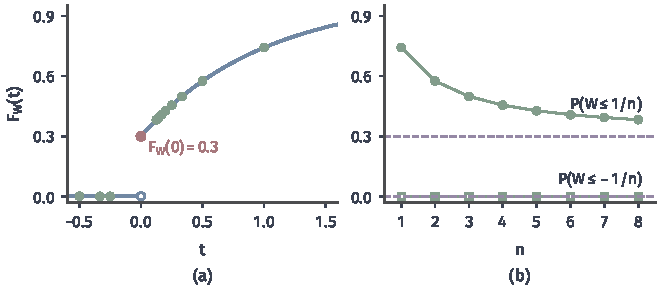
\includegraphics[width=112mm]{figures/07-probability/02-measure-theoretic-probability/matplotlib/pspace-continuity/figure.pdf}
  \caption{等待时间$W$的分布函数与概率的连续性。(a)蓝线是$F_W$，空心点是$0$处的左极限，红点是$F_W(0)=0.3$；右侧绿点是$t=1/n$处的值，左侧绿点是$t=-1/n$处的值。(b)绿色实心点是递减事件$\{W\leq1/n\}$的概率，趋于$0.3$；空心方块是递增事件$\{W\leq-1/n\}$的概率，恒为$0$。紫色虚线是两个极限。}
  \label{fig:pspace-continuity}
\end{BookInlineFigure}

\paragraph{已有模型怎样成为概率空间}
第一部分的每个模型都可以写成一个概率空间，只是事件族和概率的给法不同。

古典模型取$\Omega$有限，$\mathcal{F}$为全部子集，$\mathbb{P}(A)=\lvert A\rvert/\lvert\Omega\rvert$。有限个集合不可能有无穷多个两两不交的非空成员，可数可加性归结为有限可加性，也就是计数的加法。

概率表取$\Omega$可数，$\mathcal{F}$为全部子集，给每个$\omega$一个$p(\omega)\geq0$，且$\sum_{\omega}p(\omega)=1$，令$\mathbb{P}(A)=\sum_{\omega\in A}p(\omega)$。对两两不交的$A_1,A_2,\dots$，
\[
  \mathbb{P}\Bigl(\bigcup_{k}A_k\Bigr)=\sum_{k}\sum_{\omega\in A_k}p(\omega)=\sum_{k}\mathbb{P}(A_k),
\]
第一个等号把并集中的点按所属的$A_k$分组。非负项级数可以任意重排、分组而和不变，这就是可数可加性。

密度模型取$\Omega=\mathbb{R}$，$\mathcal{F}=\mathcal{B}(\mathbb{R})$。给定非负Borel函数$f$且$\int_{\mathbb{R}}f\,\mathrm{d}\lambda=1$，其中$\lambda$是Lebesgue测度，令
\begin{equation}
  \mathbb{P}(A)=\int_{A}f\,\mathrm{d}\lambda,\qquad A\in\mathcal{B}(\mathbb{R}).
  \label{eq:pspace-density-model}
\end{equation}
对两两不交的$A_k$，被积函数可以逐项拆开：
\[
  \mathbf{1}_{\bigcup_kA_k}f=\sum_k\mathbf{1}_{A_k}f,
\]
右边的部分和是递增的非负函数列。由单调收敛定理，积分与求和可以交换，于是式~\eqref{eq:pspace-density-model}可数可加。在区间上，这个积分与第一部分的黎曼积分（含反常积分）一致，可参考\BookChapterRef{chap:integration}{卷四第6章“积分”}。

混合模型把两者相加。式~\eqref{eq:pspace-waiting-law}中，$A\mapsto\mathbf{1}_{A}(0)$是$0$处的单点测度，第二项是密度为$\mathrm{e}^{-t}\mathbf{1}_{\{t>0\}}$的测度。非负系数的测度之和仍是测度，总质量$0.3+0.7=1$，所以$P_W$是概率测度。单点$\{0\}$和各种区间在同一个$\mathcal{B}(\mathbb{R})$中，可以一起运算。

\paragraph{由分布函数给出的模型}
Cantor分布既没有概率表也没有密度，它只有分布函数。第~\ref{chap:random-variables}章说过，满足三条性质的函数都可以用来规定模型；现在可以说清这句话的含义。

\begin{theorem}[分布函数确定实轴上的概率]
\label{thm:pspace-cdf-measure}
设$F:\mathbb{R}\to[0,1]$单调不减、右连续，且$\lim_{x\to-\infty}F(x)=0$，$\lim_{x\to+\infty}F(x)=1$。则$(\mathbb{R},\mathcal{B}(\mathbb{R}))$上存在唯一的概率测度$P$，使得
\begin{equation}
  P\bigl((-\infty,x]\bigr)=F(x),\qquad x\in\mathbb{R}.
  \label{eq:pspace-cdf-measure}
\end{equation}
\end{theorem}

\begin{proof}
存在性就是卷四的Stieltjes测度定理：对单调不减、右连续的$F$，存在$\mathcal{B}(\mathbb{R})$上的测度$P$，使$P((a,b])=F(b)-F(a)$对一切$a<b$成立。令$a\to-\infty$，由连续性得
\[
  P\bigl((-\infty,b]\bigr)=\lim_{a\to-\infty}\bigl(F(b)-F(a)\bigr)=F(b).
\]
再令$b\to+\infty$得$P(\mathbb{R})=1$。

唯一性用卷四的$\pi$--$\lambda$定理。半直线族$\{(-\infty,x]:x\in\mathbb{R}\}$对有限交封闭，因为$(-\infty,x]\cap(-\infty,y]=(-\infty,\min\{x,y\}]$，所以它是$\pi$系统，并且生成$\mathcal{B}(\mathbb{R})$。两个概率测度若在一个生成$\sigma$代数的$\pi$系统上一致，就在整个$\sigma$代数上一致。满足式~\eqref{eq:pspace-cdf-measure}的两个概率测度在半直线上一致，因此相同。
\end{proof}

这个定理有两层意思。唯一性说，分布函数记录了实轴上全部Borel集的概率，而不只是区间的概率；第一部分只能从$F$读出区间的概率，现在知道其余集合的概率也已被确定。存在性说，Cantor函数确实对应一个概率测度，第~\ref{chap:random-variables}章的Cantor分布不是一个只有分布函数的“形式对象”。

\paragraph{单点的概率与总概率}
木棍上的均匀随机点由$\Omega=[0,1)$、$\mathcal{F}=\mathcal{B}([0,1))$和长度测度$\lambda$给出。每个单点的概率为零：对任意$h>0$，$\{x\}\subseteq[x,x+h)$，所以$\lambda(\{x\})\leq h$，再令$h\to0$。由可数可加性，任何可数集的概率也为零，特别地
\[
  \mathbb{P}\bigl(\mathbb{Q}\cap[0,1)\bigr)=\sum_{q}\lambda(\{q\})=0 .
\]

不借助单点的结论，也可以直接看到有理数集“太稀”。把有理数排成一列$q_1,q_2,\dots$，用以$q_k$为中心、长$\varepsilon/2^{k}$的区间覆盖它，总长度不超过$\varepsilon$（图~\ref{fig:pspace-rational-cover}）。$\varepsilon$可以任意小，所以有理数集的概率为零，尽管有理数在$[0,1)$中处处稠密。

\begin{BookInlineFigure}
  \centering
  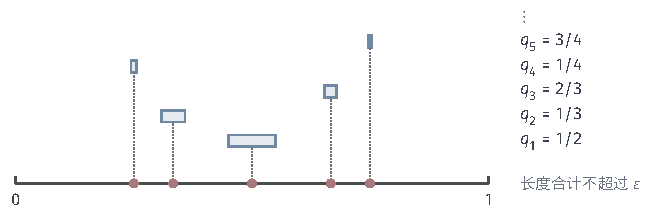
\includegraphics[width=104mm]{figures/07-probability/02-measure-theoretic-probability/tikz/pspace-rational-cover/figure.pdf}
  \caption{用总长度不超过$\varepsilon$的区间覆盖$[0,1)$中的有理数，这里$\varepsilon=0.2$。红点是按某种次序排列的前五个有理数$q_k$，浅蓝区间以$q_k$为中心，长$\varepsilon/2^{k}$，依次为$0.1,0.05,0.025,\dots$，越来越短。}
  \label{fig:pspace-rational-cover}
\end{BookInlineFigure}

另一方面，$[0,1)$是它的单点之并，每个单点的概率都是$0$，总概率却是$1$。这并不矛盾。可数可加性只对可数个事件成立，而$[0,1)$的点不可数。若硬要对不可数个零相加，把和定义为所有有限部分和的上确界，结果是$0$而不是$1$。所以“总概率等于各点概率之和”只在可数情形成立。

质量的比喻能帮助理解这一点。一根质量为$1$、均匀的细棒，任何一点处都没有质量，质量只存在于有长度的小段上；密度描述的是单位长度上的质量，而不是某个点的质量。概率表适合把质量集中在可数个点上的模型，长度测度与密度适合把质量连续铺开的模型，$W$的分布兼有两者。概率测度的语言不偏向任何一种：它只规定事件的概率，并要求对可数个不交事件可加。

\subsection{零概率与几乎必然}
\label{sec:pspace-null-events}

在古典模型中，若每个样本点的概率都为正，那么概率为零的事件只有空集。连续模型打破了这一点：$\{U=1/2\}$非空，$U$完全可能落在$1/2$，可它的概率是$0$。需要一套说法，既承认这些事件可能发生，又在计算中把它们略去。

\begin{definition}[零概率事件与几乎必然]
\label{def:pspace-almost-sure}
设$(\Omega,\mathcal{F},\mathbb{P})$是概率空间。满足$\mathbb{P}(N)=0$的事件$N$称为\term{零概率事件}（null event）。若一个关于样本点的陈述不成立的点全体包含于某个零概率事件，则称该陈述\term{几乎必然}（almost surely）成立，简记为a.s.。
\end{definition}

这就是卷四“几乎处处”在概率测度下的说法。定义只要求失败点集\emph{包含于}一个零概率事件，因为失败点集本身未必在$\mathcal{F}$中；下一小节的完备化讨论这种情形。等价地，若陈述成立的点集是事件，几乎必然成立就是它的概率等于$1$。

\paragraph{不可能与零概率}
空集是不可能事件，它在任何结果下都不发生。零概率事件可以发生，只是在概率的计算中不占质量。$U$是均匀随机点，$\{U=1/2\}$、$\{U\in\mathbb{Q}\}$都是非空的零概率事件，相应地，“$U\neq1/2$”“$U$是无理数”都几乎必然成立，但不是必然成立。等待时间的例子中，$\{W=1\}$概率为零，$\{W=0\}$的概率却是$0.3$；哪些单点是零概率事件，由概率测度决定，与样本点本身无关。

零概率事件还依赖于所用的概率。在$\Omega=\{0,1\}$上，若$\mathbb{P}(\{1\})=0$，“结果是$0$”几乎必然成立；换成$\mathbb{P}(\{1\})=1/2$，同一句话就不成立了。所以说“几乎必然”时，必须清楚是相对于哪个概率测度。

\paragraph{可数个几乎必然的陈述}
几乎必然的陈述可以放心地合并可数次，这是它最常用的性质。

\begin{lemma}[可数个零概率事件之并]
\label{lem:pspace-countable-null}
若$N_1,N_2,\dots$都是零概率事件，则$\bigcup_kN_k$也是零概率事件。因此，可数个各自几乎必然成立的陈述，同时几乎必然成立。
\end{lemma}

\begin{proof}
由联合界，
\[
  0\leq\mathbb{P}\Bigl(\bigcup_{k}N_k\Bigr)\leq\sum_{k}\mathbb{P}(N_k)=0 .
\]
设第$k$个陈述在零概率事件$N_k$之外成立，则所有陈述在$\bigcup_kN_k$之外同时成立，而这个并集概率为零。
\end{proof}

第一个例子补上第~\ref{chap:random-vectors}章留下的一步。设$Y$与$L$是同一样本空间上的两个函数，已知对每个$\varepsilon>0$都有$\mathbb{P}(\lvert Y-L\rvert>\varepsilon)=0$。$Y$与$L$不相等，当且仅当它们相差某个$1/n$以上，所以
\[
  \{Y\neq L\}=\bigcup_{n=1}^{\infty}\bigl\{\lvert Y-L\rvert>1/n\bigr\}.
\]
右边是可数个零概率事件之并，由引理~\ref{lem:pspace-countable-null}，$\mathbb{P}(Y\neq L)=0$，即$\mathbb{P}(Y=L)=1$。这里只取$\varepsilon=1/n$这可数个值就够了，不需要对每个正数$\varepsilon$分别处理。

\paragraph{不可数个例外}
可数性不能省略。设$U$是均匀随机点，对每个$t\in[0,1)$令
\[
  X_t(\omega)=\mathbf{1}_{\{U(\omega)=t\}},
\]
即$U$恰好等于$t$时取$1$，否则取$0$。对每个固定的$t$，$X_t\neq0$的事件是$\{U=t\}$，概率为零，所以$X_t=0$几乎必然成立。

可是对每个样本点$\omega$，取$t=U(\omega)$就有$X_t(\omega)=1$。于是
\[
  \bigl\{\omega:\ X_t(\omega)=0\text{ 对一切 }t\text{ 成立}\bigr\}=\varnothing .
\]
“对每个$t$，几乎必然$X_t=0$”成立，“几乎必然对一切$t$都有$X_t=0$”却完全不成立。原因是例外事件$\{U=t\}$随$t$变化，不可数个零概率事件之并是整个$\Omega$。图~\ref{fig:pspace-uncountable-spikes}画出了三个样本点对应的函数$t\mapsto X_t(\omega)$：每条都只在一个位置有尖峰，固定任何一个时刻$t_0$去看，几乎看不到尖峰；但每条曲线都有尖峰。

\begin{BookInlineFigure}
  \centering
  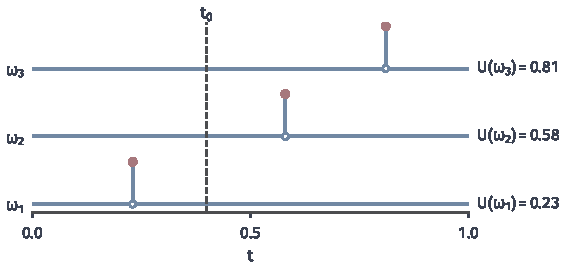
\includegraphics[width=96mm]{figures/07-probability/02-measure-theoretic-probability/matplotlib/pspace-uncountable-spikes/figure.pdf}
  \caption{$X_t=\mathbf{1}_{\{U=t\}}$在三个样本点上的取值，横轴是$t$。每条蓝线只在$t=U(\omega)$处跳到$1$（红点）。虚线是固定时刻$t_0$，它碰到尖峰的概率为零；然而每个样本点的曲线都有一个尖峰。}
  \label{fig:pspace-uncountable-spikes}
\end{BookInlineFigure}

要从“每个$t$几乎必然”推出“几乎必然对一切$t$”，需要额外的结构。例如，若已知每条曲线$t\mapsto X_t(\omega)$都连续，就只需检查可数个有理数时刻：它们在零概率事件之外同时为零，连续性再把结论推到所有$t$。上面的$X_t$不连续，这条路走不通。以连续时间为指标的随机对象经常遇到这个问题，本章只处理可数个陈述。

\subsection{完备化}
\label{sec:pspace-completion}

几乎必然的陈述允许在零概率事件上随意修改。修改以后的对象还在原来的事件族里吗？先看一个小例子。

\paragraph{修改可能破坏可测性}
取$\Omega=\{1,2,3\}$，事件族与概率为
\[
  \mathcal{F}=\bigl\{\varnothing,\{1\},\{2,3\},\Omega\bigr\},\qquad \mathbb{P}(\{1\})=1,\quad \mathbb{P}(\{2,3\})=0 .
\]这个事件族只能区分“结果是$1$”与“结果在$\{2,3\}$中”。按卷四的说法，函数$X:\Omega\to\mathbb{R}$\emph{可测}是指对每个Borel集$B$，$\{X\in B\}\in\mathcal{F}$；第~\ref{sec:pspace-random-objects}节将把这样的函数称为随机变量。

$X\equiv0$可测，因为它的每个原像都是$\varnothing$或$\Omega$。令$X'=\mathbf{1}_{\{2\}}$，它与$X$只在点$2$不同，而$\{2\}\subseteq\{2,3\}$包含于零概率事件，所以$X'=X$几乎必然成立。然而$\{X'=1\}=\{2\}\notin\mathcal{F}$，$X'$不可测。两个函数几乎必然相等，一个可测、一个不可测，问题出在$\mathcal{F}$不含零概率事件$\{2,3\}$的子集。

\paragraph{完备化的定义}
卷四的完备化正好补上这些集合。称概率空间$(\Omega,\mathcal{F},\mathbb{P})$\term{完备概率空间}（complete probability space），若每个零概率事件的每个子集都属于$\mathcal{F}$。对任意概率空间，令
\begin{equation}
  \overline{\mathcal{F}}=\{A\cup M:\ A\in\mathcal{F},\ M\subseteq N\text{ 对某个零概率事件 }N\},\qquad \overline{\mathbb{P}}(A\cup M)=\mathbb{P}(A).
  \label{eq:pspace-completion}
\end{equation}
卷四证明了：$\overline{\mathcal{F}}$是包含$\mathcal{F}$的$\sigma$代数，$\overline{\mathbb{P}}$与表示方式无关，是$\overline{\mathcal{F}}$上的概率测度，在$\mathcal{F}$上与$\mathbb{P}$一致，并且$(\Omega,\overline{\mathcal{F}},\overline{\mathbb{P}})$完备。

在上面的例子中，零概率事件只有$\varnothing$和$\{2,3\}$，它们的子集$\{2\}$、$\{3\}$被补入，再与$\{1\}$取并，得到全部$8$个子集（图~\ref{fig:pspace-completion}）。新补入的事件中，含点$1$的概率为$1$，不含点$1$的概率为$0$；原有$4$个事件的概率不变。

\begin{BookInlineFigure}
  \centering
  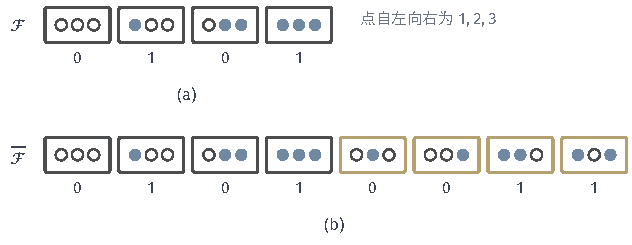
\includegraphics[width=107mm]{figures/07-probability/02-measure-theoretic-probability/tikz/pspace-completion/figure.pdf}
  \caption{三点样本空间的完备化。每个方框是一个事件，实心点表示该点属于事件，下方数字是概率。(a)原事件族$\mathcal{F}$只有$4$个事件；(b)完备化补入零概率事件$\{2,3\}$的子集及其与$\{1\}$的并（黄框），共$8$个事件，原有事件的概率不变。}
  \label{fig:pspace-completion}
\end{BookInlineFigure}

\paragraph{完备空间中的修改}
在完备的概率空间里，零概率事件上的修改不会破坏可测性。

\begin{theorem}[零概率修改保持可测性]
\label{thm:pspace-modification}
设$(\Omega,\mathcal{F},\mathbb{P})$完备，$X:\Omega\to\mathbb{R}$可测，$X':\Omega\to\mathbb{R}$满足：存在零概率事件$N$，使得在$N$之外$X'=X$。则$X'$可测，且对每个Borel集$B$，
\begin{equation}
  \mathbb{P}(X'\in B)=\mathbb{P}(X\in B).
  \label{eq:pspace-modification}
\end{equation}
\end{theorem}

\begin{proof}
把$\{X'\in B\}$按是否落在$N$中分成两块：
\[
  \{X'\in B\}=\bigl(\{X\in B\}\cap N^{\mathrm{c}}\bigr)\cup\bigl(\{X'\in B\}\cap N\bigr).
\]
在$N^{\mathrm{c}}$上$X'=X$，所以第一块等于$\{X\in B\}\cap N^{\mathrm{c}}$，它是两个事件之交，属于$\mathcal{F}$。第二块包含于零概率事件$N$，由完备性也属于$\mathcal{F}$，且概率为零。所以$\{X'\in B\}\in\mathcal{F}$，并且
\[
  \mathbb{P}(X'\in B)=\mathbb{P}\bigl(\{X\in B\}\cap N^{\mathrm{c}}\bigr)=\mathbb{P}(X\in B),
\]
最后一步是因为$\{X\in B\}$与$\{X\in B\}\cap N^{\mathrm{c}}$相差的部分包含于$N$。
\end{proof}

木棍上的随机点就有这样的例子。卷四指出，$\mathcal{B}([0,1))$关于长度的完备化是Lebesgue可测集族。Cantor集的长度为零，在完备化后它的每个子集都是事件，概率都是零，其中包括不是Borel集的子集。于是，把一个随机变量在Cantor集的任意子集上改掉，得到的函数在完备空间中仍然可测，所有概率都不变。

\paragraph{完备化不做的事}
完备化只是把“包含于零概率事件”的集合补进来并赋予概率零，它不改变原有事件的概率，也不会让任何零概率事件变成正概率事件。特别地，它不能帮助我们以零概率事件为条件。给定$U=1/2$时某事件的条件概率，按第~\ref{chap:classical-probability}章的定义是
\[
  \mathbb{P}(A\mid U=1/2)=\frac{\mathbb{P}(A\cap\{U=1/2\})}{\mathbb{P}(U=1/2)},
\]
分母为零，完备化前后都一样。给定连续观测值求条件规律，要用第~\ref{chap:conditional-expectation}章和第~\ref{chap:conditional-distributions}章的办法。

完备化也有代价。零概率事件依赖于概率测度，对一个测度完备的事件族，换一个测度就未必完备；同时讨论多个概率测度时，通常保留原来的事件族。对取值空间，惯例是使用Borel $\sigma$代数而不完备化：卷四说明过，Lebesgue可测函数与连续函数的复合未必Lebesgue可测，取值一侧若换成更大的事件族，复合运算就可能失去可测性。本章约定：样本空间一侧需要时可以完备化，取值空间一律使用Borel $\sigma$代数。
